\chapter{Conditioning of Least Squares Problems} 
The conditioning of least squares problems is a subtle topic, combining the conditioning of square systems of equations with the geometry of orthogonal projection. It is important because it has nontrivial implications for the stability of least squares algorithms.

\section{Four Conditioning Problems}
We return to the linear least squares problems. We assume $\|\cdot \| = \|\cdot \|_2$ in this chapter and the matrix is of full rank: 
\begin{align}
    \label{eq: LSp} 
    \text{ Given } A\in \CC^{m\times n} \text{ of full rank, } m\ge n, b\in \CC^m, \\ 
    \text{ find } x\in \CC^n \text{ such that } \|b-Ax\| \text{ is minimized. } \notag 
\end{align}

The solution is given by, 
\begin{equation}
    \label{eq: solu of LS} 
    x = A^\dagger b, \quad y = Pb. 
\end{equation}

We consider the conditioning of \eqref{eq: LSp} w.r.t. perturbations. Conditioning pertains to the sensitivity of solutions to perturbations in data. The data for the problem are matrix $A$ and the vector $b$. The solution can be $x$ or $y$. Thus, 
\[
    \text{ Data: }A,b, \quad \text{ Solution: } x,y. 
\]
Together, these two paris of choices defined four conditioning questions. 

\section{Theorem}
The results are expressed in terms of three dimensionless parameters: 
\begin{itemize}
    \item Given a matrix $A$, the condition number $\kappa(A) = \|A\| \|A^\dagger\| = \frac{\sigma_1}{\sigma_n}.$ 
    \item The angle between $y$ and $b$: $ \theta  = \cos^{-1} \frac{\|y\|}{\|b\|} $ . 
    \item How much $\|y\|$ falls short of its maximum possible value:  $\eta = \frac{\|A\| \|x\|}{\|y\|} = \frac{\|A\| \|x\|}{\|Ax\|}$. 
\end{itemize}
These parameters lie in the ranges: 
\[
    1 \leq \kappa(A)<\infty, \quad 0 \leq \theta \leq \pi / 2, \quad 1 \leq \eta \leq \kappa(A). 
\]


%────────────────────────────────────────
\begin{theorem}
[Conditioning of LS]
\label{thm: Conditioning of LS}
Let $b\in \CC^m$ and $A\in \CC^{m\times n}$ of full rank be fixed. The LS problem \eqref{eq: LSp} has the following 2-norm condition numbers describing the sensitivities of $y$ and $x$ to perturbations in $b$ and $A$: 

%────────────────────────────────────────
\begin{table}[H]
    \centering
    \begin{tabular}{|c|c|c|}
    \hline 
    & $y$ &$x$ \\ 
    \hline \xrowht{20pt}
    $b$ & $ \frac{1}{\cos \theta} $ & $\frac{\kappa(A)}{\eta \cos \theta}$ \\ 
    \hline \xrowht{20pt}
    $A$ & $\frac{\kappa(A)}{\cos \theta}$ & $\kappa(A) + \frac{\kappa(A)^2 \tan \theta }{\eta}$ \\ 
    \hline
    \end{tabular}
\end{table}
%────────────────────────────────────────
The results in the first row are exact, being attained for certain perturbations $\delta b$, and the results in the second row are upper bounds. 
\end{theorem}
%────────────────────────────────────────

%────────────────────────────────────────
\begin{note}
In the special case $m=n$, \eqref{eq: LSp} reduces to a square, nonsingular system of equations, with $\theta =0$. In this case, the numbers in the second column of the theorem reduces $\kappa(A)/\eta$ and $\kappa(A)$, which are the results \eqref{eq: cond of Ainv} and \eqref{eq: cond of purturb A} derived earlier.  
\end{note}
%────────────────────────────────────────

\section{Transformation to a Diagonal Matrix} 
Assume $A = U\Sigma V^*$, since perturbations are measures in the 2-norm, we can assume $A=\Sigma$ and write 
\[
    A=\left[\begin{array}{cccc}
        \sigma_1 & & & \\
        & \sigma_2 & & \\
        & & \ddots & \\
        & & & \sigma_n \\
        & & &
        \end{array}\right]=\left[\begin{array}{c}
        A_1 \\
        0
        \end{array}\right]. 
\]

Assume $b = \begin{bmatrix}
     b_1 \\
     b_2 \\
\end{bmatrix}$, then the projection $y=Pb$ is  $y = \begin{bmatrix}
         b_1 \\
         0 \\
    \end{bmatrix}.$   
Hence, $Ax=y$ is 
\[
    \begin{bmatrix}
         A_1 \\
         0 \\
    \end{bmatrix} x = \begin{bmatrix}
         b_1 \\
         0 \\
    \end{bmatrix},  
\]
which implies $   x = A_1^{-1} b_1. $
It's easy to find that 
\[
    P = \begin{bmatrix}
        I &  0 \\
        0 &  0 \\
    \end{bmatrix}, \quad A^\dagger = \begin{bmatrix}
        A_1^{-1}  &  0 \\
    \end{bmatrix}.   
\]

\section{Sensitivity of $y$ to Perturbations in $b$}  
Note that $y= Pb$ and the Jacobian is $P$ itself. Hence, the condition number of $y$ w.r.t. perturbations in $b$ is: 
\[
    \kappa_{b mapsto y} = \frac{\|P\|}{\|y\|/ \|b\|} = \frac{1}{\cos \theta}. 
\]
 The condition number is realized when $\delta b$ is zero except in the first $n$ entries. 

 \section{Sensitivity of $x$ to Perturbations in $b$} 
 The relationship between $b$ and $x$ is $x= A^\dagger b$. Hence, 
 \[
    \kappa_{b\mapsto x} = \frac{\|A^\dagger\|}{\|x\|/ \|b\|} = \|A^\dagger\| \frac{\|b\|}{\|y\|}\frac{\|y\|}{\|A\| \|x\|}\|A\| = \frac{\kappa(A)}{\eta  \cos \theta }. 
 \]

 Here the condition number is realized by perturbation $\delta  b$ sastisfying $ \|A^\dagger (\delta  b)\| = \|A^\dagger\| \|\delta  b\| = \|\delta  b \|/ \sigma _n$, which means $\delta b= e_n$. 

 \section{Tilting the range of $A$} 
 The analysis of perturbations in $A$ is a nonlinear problem and more subtle. We could proceed by calculating Jacobians algebraically, but instead, we shall take a geometric view. Our starting point is the observation that perturbations in $A$ affect the least squares problem in two ways: 
 \begin{itemize}
    \item They distort the mapping of $\CC^n$ onto $\range(A)$; 
    \item They alter $\range(A)$ itself. 
 \end{itemize}
Let us consider this latter effect now.  

We can visualize slight changes in $\range(A)$ as small ``tiltings'' of this space. The question is, \textbf{What is the maximum angle of tilt $\delta \alpha $ that can be imparted by a small perturbation $\delta A$?} The answer can be determined as follows.  The image under $A$ of the unit $n$-sphere is a hyperellipse that lies flat in $\range(A)$. To change $\range(A)$ as efficiently as possible, we grasp a point $p=Av$ on the hyperellipse and nudge it in a direction $\delta p$ orthogonal to $\range(A)$. A matrix perturbation that achieves this most efficient is $\delta  A = (\delta p) v^*$,  which gives $(\delta A) v = \delta  p$ with $\|\delta A\| = \|\delta p\|$. 

Now it's clear that to obtain the maximum tilt with a given $\|\delta p\|$, we should take $p$ to be as close to the origin as possible. That is, we want $p=\sigma _n u_n$, where $\sigma _n$ is the smallest singular value of $A$ and $u_n$ is the corresponding left singular vector. With $A$ in the  diagonal form, $p$ is equal to the last column of $A$ and $v^*$ is the $n$-vector $(0,0,\ldots ,0,1)$, and $\delta A$ is a perturbation of the entries of $A$ below the diagonal in this column.  Such a perturbation tilts $\range(A)$ by the angle $\delta \alpha $ given by $\tan (\delta \alpha ) = \|\delta p\|/ \sigma _n$. Since $\|\delta p\| = \|\delta A\|$ and $\delta \alpha  \le \tan (\delta \alpha )$, we have 
\begin{equation}
    \label{eq: delta alpah to delta a}
    \delta \alpha  \le \frac{\|\delta A\|}{\sigma _n}= \frac{\|\delta A\|}{\|A\|} \kappa (A), 
\end{equation}
wit equality attained for choices $\delta A$ of this kind just described.  

\section{Sensitivity of $y$ to Perturbations in $A$} 
We begin with the left-hand entry in the second row of the table in \autoref{thm: Conditioning of LS}. Since $y$ is the orthogonal projection of $b$ onto $\range(A)$, it's determined by $b$ and $\range(A)$ alone. Therefore, to analyze the sensitivity of $y$ to perturbations in $A$, we can simply study the effect on $y$ of tilting $\range(A)$ by some angle $\delta \alpha $.  

%────────────────────────────────────────
\begin{figure}[H]
    \centering
    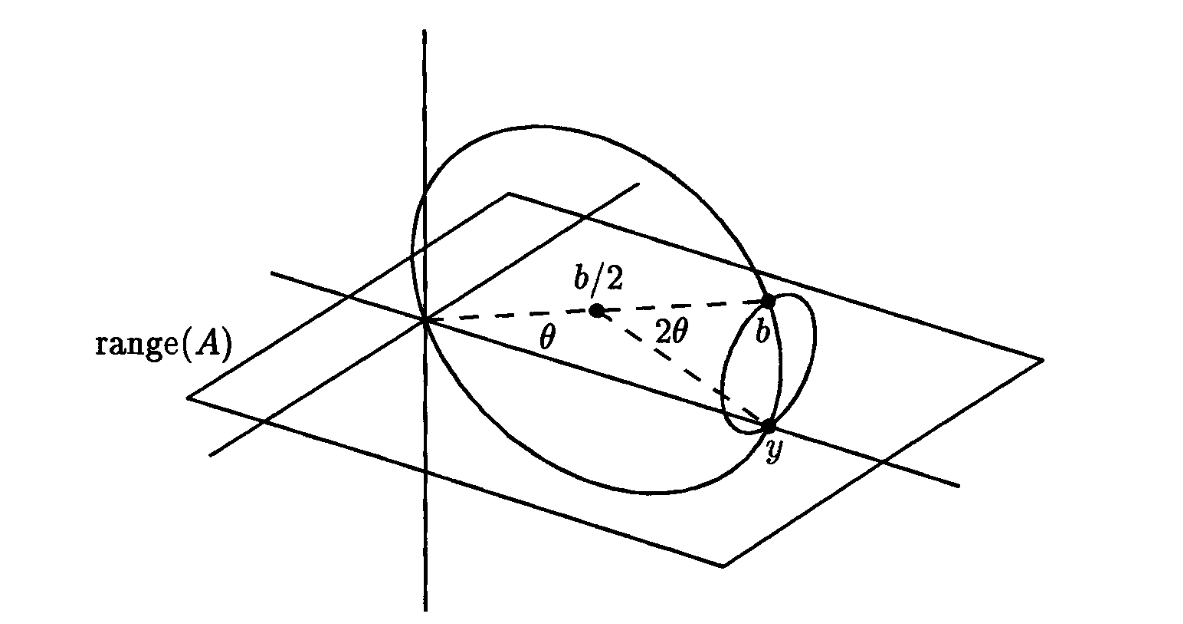
\includegraphics[width=0.8\textwidth]{figures/18-2.png}
    \label{fig: 18.2}
    \caption{Two circles on the sphere along which $y$ moves as $\range(A)$ varies. The large circle, of radius $\|b\|/2$, corresponds to tilting $\range(A)$ in the plane $0-b-y$, and the small circle of radius $(\|b\|/2)\sin \theta $, corresponds to tilting it in an orthogonal direction. However $\range(A)$ is tilted, $y$ remains on the sphere of radius $\|b\|/2$ centered at $\frac{b}{2}$.}
\end{figure}
%────────────────────────────────────────

An elegant geometrical property becomes apparent when we imagine fixing $b$ and watching $y$ vary as $\range(A)$ is tilted. No matter how $\range(A)$ is tilted, the vector $y\in \range(A)$ must always be orthogonal to $y-b$. That is, the line $b-y$ must lie at right angles to the line $0-y$. In other words, as $\range(A)$ is adjusted, $y$ moves along the sphere of radius $\|b\|/2$ centered at the point $b /2$. 

Tilting $\range(A)$ in the plane $0-b-y$ by an angle $\delta \alpha $ changes the angle $2\theta $ at the central point $\frac{b}{2}$ by $2\delta \alpha $. Thus the corresponding perturbation $\delta y$ is the base of an isosceles triangle with central angle $2\delta \alpha $ and edge length $\|b\|/2$. This implies $\|\delta y\| = \|b\| \sin (\delta \alpha )$. Tilting $\range(A)$ in any other direction results in a similar geometry in a different plane and perturbations smaller by a factor as small as $\sin \theta $. Thus for arbitrary perturbations by an angle $\delta \alpha $ we have 
\begin{equation}
    \label{eq: y to A} 
    \|\delta  y \|\le \|b\| \sin (\delta \alpha ) \le \|b\| \delta \alpha . 
\end{equation}

By the definition of $\theta$ and \eqref{eq: delta alpah to delta a}, we have 
\begin{equation}
    \label{eq: sensi y to A} 
    \|\delta y\| \le \frac{ \|\delta A\|}{\|A\|}\kappa(A) \cdot \frac{\|y\|}{\cos \theta } \Rightarrow \frac{\|\delta y\|}{\|y\|}\Big / \frac{\|\delta A\|}{\|A\|} \le \frac{\kappa(A)}{\cos \theta }. 
\end{equation}

\section{Sensitivity of $x$ to Perturbations in $A$} 

We are now ready to analyze the most interesting relationship of \autoref{thm: Conditioning of LS}: the sensitivity of $x$ to perturbations in $A$. A perturbation $\delta A$ splits naturally into two parts: one part $\delta A_1$ in the fist $n$ rows of $A$, and another part $\delta  A_2$ in the remaining $m-n$ rows: 
\[
    \delta A=\left[\begin{array}{l}
        \delta A_1 \\
        \delta A_2
        \end{array}\right]=\left[\begin{array}{c}
        \delta A_1 \\
        0
        \end{array}\right]+\left[\begin{array}{c}
        0 \\
        \delta A_2
        \end{array}\right]. 
\]
First, let us consider the effect of perturbations $\delta A_1$. Such a perturbation changes the mapping of $A$ in its range, but not $\range(A)$ itself or $y$. It perturbs $A_1$ by $\delta A_1$ in the square system \eqref{eq: LSp} without changing $b_1$. The condition for such perturbations is given by \eqref{eq: cond of purturb A}, which here takes the form 
\begin{equation}
    \label{eq: delta A1} 
    \frac{\|\delta x\|}{\|x\|} / \frac{\left\|\delta A_1\right\|}{\|A\|} \leq \kappa\left(A_1\right)=\kappa(A). 
\end{equation}

Next we consider the effect of perturbations $\delta A_2$. Such a perturbation tilts $\range(A)$ without changing the mapping of $A$ within this space. The point $y$ and thus the vector $b_1$ are perturbed, but not $A_1$. This corresponding to perturbing $b_1$ without changing $A_1$. The condition number for such perturbation is given by \eqref{eq: cond of Ainv}, which takes the form 
\begin{equation}
    \frac{\|\delta x\|}{\|x\|} / \frac{\left\|\delta b_1\right\|}{\left\|b_1\right\|} \leq \frac{\kappa\left(A_1\right)}{\eta\left(A_1 ; x\right)}=\frac{\kappa(A)}{\eta} .
\end{equation}

To finish the argument, we need to relate $\delta b_1$ to $\delta A_2$. Now the vector $b_1$ is $y$ expressed in the coordinates of $\range(A)$.  Therefore, the only changes in $y$ that realized as changes in $b_1$ are those that lie parallel to $\range(A)$; orthogonal changes have no effect. In particular, if $\operatorname{range}(A)$ is tilted by an angle $\delta \alpha$ in the plane $0-b-y$, the resulting perturbation $\delta y$ lies not parallel to range $(A)$ but at an angle $\pi / 2-\theta$. Consequently, the change in $b_1$ satisfies $\left\|\delta b_1\right\|=\sin \theta\|\delta y\|$. By $\eqref{eq: y to A}$, we therefore have
\begin{align*}
\left\|\delta b_1\right\| \leq(\|b\| \delta \alpha) \sin \theta
\end{align*}
Curiously, if range $(A)$ is tilted in a direction orthogonal to the plane $0-b-y$, we obtain the same bound, but for a different reason. Now $\delta y$ is parallel to range $(A)$, but it is a factor of $\sin \theta$ smaller, as discussed above in connection with Figure 18.2. Thus we have $\|\delta y\| \leq(\|b\| \delta \alpha) \sin \theta$, and since $\left\|\delta b_1\right\| \leq\|\delta y\|$, we again arrive at the same result.

All the pieces are now in place. Since $\left\|b_1\right\|=\|b\| \cos \theta$, we can rewrite before as
\begin{align*}
\frac{\left\|\delta b_1\right\|}{\left\|b_1\right\|} \leq(\delta \alpha) \tan \theta
\end{align*}
Relating $\delta \alpha$ to $\left\|\delta A_2\right\|$ by \eqref{eq: delta alpah to delta a} and combining the previous results, we obtain
\begin{align*}
\frac{\|\delta x\|}{\|x\|} / \frac{\left\|\delta A_2\right\|}{\|A\|} \leq \frac{\kappa(A)^2 \tan \theta}{\eta} .
\end{align*}
Adding this to \eqref{eq: delta A1} establishes the lower-right result of Theorem~\ref{thm: Conditioning of LS}.